\documentclass[11pt,a4paper]{article}
\usepackage[utf8]{inputenc}
\usepackage[spanish]{babel}
\usepackage{amsmath}
\usepackage{amsfonts}
\usepackage{amssymb}
\usepackage{makeidx}
\usepackage{graphicx}
\usepackage{lmodern}
\usepackage{kpfonts}
\usepackage{parskip}
\usepackage[left=2cm,right=2cm,top=2cm,bottom=2cm]{geometry}
\author{Miguel Angel Xamie Diaz Fuentes}
\begin{document}
\begin{center}
\begin{LARGE}
\textbf{INGENIERÍA MECATRÓNICA}\\
\end{LARGE}
{\large Sistemas Eletrónicos De Interfaz}\\
\begin{figure}[hbtp]
\centering

\includegraphics[scale=0.80]{UPZMG_Mecatr_nica.png}
\end{figure} 
\begin{center}
\begin{LARGE}
EV-2-6 CONSTRUIR UNA AMPLIFICACION CON CONEXION DARLINGTON
\end{LARGE}
\end{center}

\begin{Large}
\textbf{Alumno}
\\\textit{Miguel Angel Xamie Diaz Fuentes}
\textbf{\\Maestro}
\\\textit{Morán Garabito Carlos Enrique}
\textbf{\\Fecha de Entrega}
\\\textit{06/11/2019}
\textbf{\\Grupo}
\\\textit{4-B}\\
\textbf{Período Cuatrimestral}\\
\textit{2019-Septiembre-Diciembre}
\\
\end{Large}

\end{center}

\footnote{Universidad Politécnica De La Zona Metropolitana De Guadalajara} 

\newpage

\section{Desarrollo}

\textbf{Que es un Darlington?
}

El transistor Darlington es un dispositivo semiconductor que combina dos transistores bipolares en una configuración tipo Darlington en un único dispositivo (a veces llamado par Darlington). Esta conexión permite que la corriente amplificada por el primer transistor ingrese a la base del segundo transistor y sea nuevamente amplificada.

Un transistor Darlington se comporta como un transistor ordinario, es decir, posee base, colector y emisor y puede ser considerado como un único transistor con una ganancia de corriente equivalente. Generalmente suele considerarse que la ganancia de un transistor Darlington es aproximadamente el producto de las ganancias de los transistores que lo componen. 

\textbf{CALCULO DE LA GANANCIA DE CORRIENTE}

Las corrientes del transistor Darlington pueden expresarse en función de las corrientes de los transistores que lo componen de la siguiente manera. 

$ I_{BD} = I_{B1} $
$ I_{CD} = I_{C1} + I_{C2} $
$ I_{ED} = I_{E2} $

A su vez, según las relaciones entre las corrientes de un transistor individual, es posible obtener la corriente de colector del par Darlington. 

$ I_{CD} = I_{C1} + I_{C2} = I_{B1} * B_1 + I_{IB2} * B_2 = 1_{B1} * B_1 + 1_{E1} * B_2 = I_{B1} * B1 + 1_{B1}$

$ I_{CD} = I_{B1} * (B1 * B2 + B1 + B2)  $

Es posible reexpresar esta última ecuación para obtener la ganancia BD del transistor Darlington a partir de la definición de dicho parámetro y considerando lo planteado en un principio. 

$ \frac{I_{CD}}{I_{BD}} = B_D = B_1 * B_2 + B_1 + B_2 $

Si se asume que B1 y B2 son suficientemente grandes, del orden de los cientos, se puede obtener la siguiente expresión aproximada. 

$ B_D \approx B_1 * B_2 $

\textbf{Ventajas}

Esta configuración permite obtener un dispositivo que proporciona una gran ganancia de corriente, típicamente del orden de los miles.Lo cual a su vez permite controlar corrientes de magnitud importante con corrientes de base muy pequeñas.

Es posible implementar esta configuración con transistores discretos, al igual que existen pares Darlington integrados en un solo encapsulado.

Lo anterior también permite utilizar menos espacio al incluir un solo encapsulado en vez de dos por separado. 

\textbf{Desventajas}

A altas frecuencias se observa que un transistor Darlington presenta un desplazamiento de fase mucho mayor que el de un único transistor. Por lo cual utilizar configuraciones de este tipo en circuitos con realimentación negativa resulta en una mayor inestabilidad de los mismos.

Otro inconveniente es la mayor caída de tensión entre la base y el emisor. Debido a que existen dos junturas entre estos dos terminales. Por ello el voltaje base-emisor resultante es igual a la suma de las caídas de ambas junturas. Es decir, que para el valor típico de 0,7 V atribuido a los transistores de silicio, se produce una caída de 1,4 V en la configuración Darlington. 

\footnote{Universidad Politécnica De La Zona Metropolitana De Guadalajara} 

\newpage

\section{Etapas de desarrollo de la practica}

\textbf{Etapa 1}

Para realizar esta practica fue necesario complementarla con la de interfacez anterior que realizamos donde teniamos 3 interfaces que son entrada, control y salidas para poder utilizar este darlington y poder realizar el circuito dado por el profesor en clase el cual explica que su funcionamiento no debe ser muy diferente a los transistores anteriores utilizados porque la función que realiza es la misma solo que utilizaremos distintas componentes para activar este darlington.

\textbf{Etapa 2}

A continuacion podremos ver el diseño que se utiliza como base para poder realizar la practica correctamente. La primera es la parte de entrada:

\begin{figure}[hbtp]
\centering
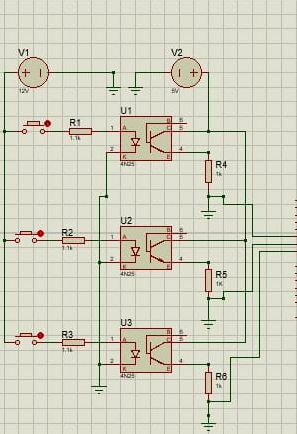
\includegraphics[scale=0.80]{entrada.png}
\end{figure}

Tenemos un voltaje de entrada para activar los optoacopladores de 12v y como salida 5v la cual al activar el pulsador son enviados a la parte de control "arduino" el cual con esta señal de entrada saca otra de salida de 5v. A continuación se muestra el código en arduino:

\footnote{Universidad Politécnica De La Zona Metropolitana De Guadalajara} 

\newpage


\begin{figure}[hbtp]
\centering
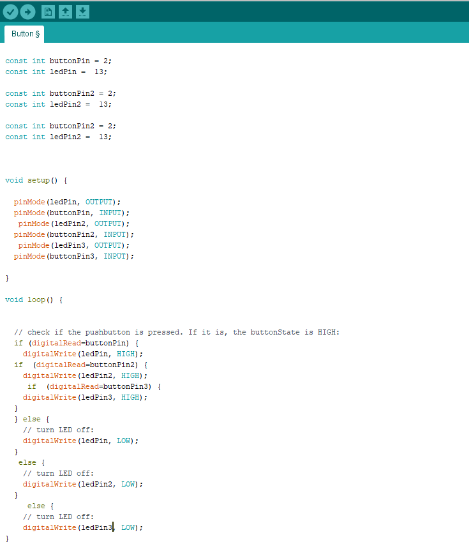
\includegraphics[scale=0.80]{codigo.png}
\end{figure}

Despues de esta salida de 5v debemos tener una circuito que actue al tener este voltaje y como anteriormente utilizamos los transistores 2N2222 en este caso serán los darlington pero con una función diferente.

A continuación tenemos las salidas:

\footnote{Universidad Politécnica De La Zona Metropolitana De Guadalajara} 

\newpage

\begin{figure}[hbtp]
\centering
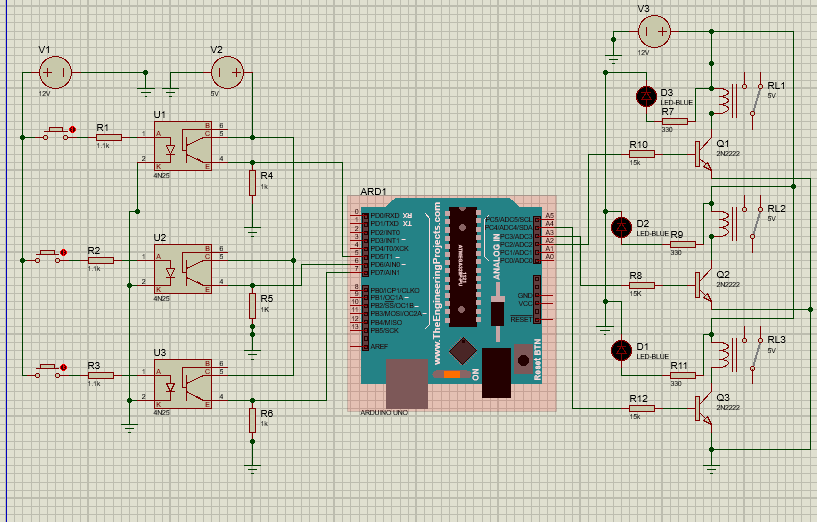
\includegraphics[scale=0.80]{3.png}
\end{figure}

De lado derecho podemos observar los transistores utilizado anteriormente, ahora se cambiaran por este símbolo del darlington:

\begin{figure}[hbtp]
\centering
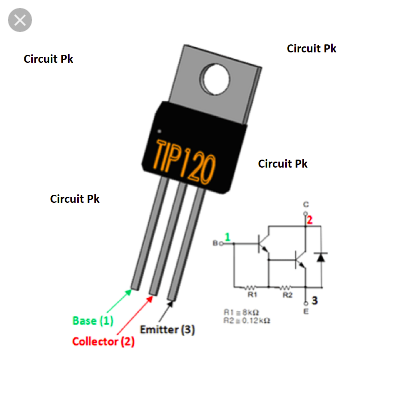
\includegraphics[scale=0.50]{1.png}
\end{figure}

\textbf{Etapa 3
}

Una vez identificado la simbología de este material el objetivo es encender un relevador y un led con un LDR. Para esto no fue cambiar algo muy muy notable solo es poner una resistencia de 1.5k en serie con el LDR y la salida de LRD a la base de este transistor. El colector le ponemos un voltaje de 5v y en el emisor va hacia la bobina y el led, las otras terminales del componente van a tierra "la bobina y el led con su resistencia" esto para que se cierre el circuito cuando se active la base.

\footnote{Universidad Politécnica De La Zona Metropolitana De Guadalajara} 

\newpage

\begin{figure}[hbtp]
\centering
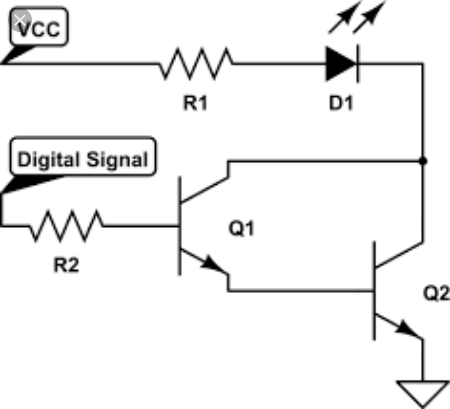
\includegraphics[scale=0.30]{5.png}
\end{figure}

Se puede observar en las siguientes imágenes el circuito ya armado el cual al detectar luz se enciende y al no detectar nada se apaga tanto el relevador como el led emisor de luz:


\begin{figure}[hbtp]
\centering
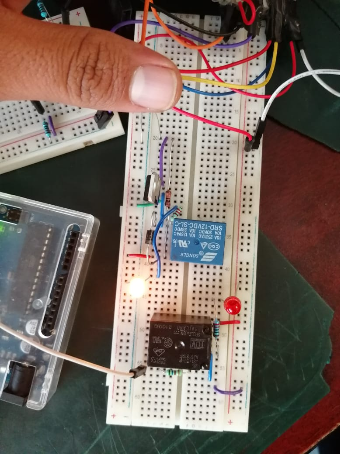
\includegraphics[scale=0.40]{6.png}
\end{figure}


\begin{figure}[hbtp]
\centering
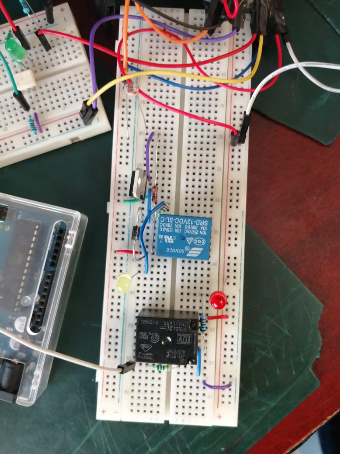
\includegraphics[scale=0.40]{7.png}
\end{figure}

\footnote{Universidad Politécnica De La Zona Metropolitana De Guadalajara} 

\newpage

\textbf{Etapa 4}

En esta etapa el actuador seria un relevador industrial en vez del led y del relevador pero su entrada de activación ya no seria por medio del ldr si no con el control de opto acoplador. La instalacion no seria complicada el único detalle que tuvimos fue que al conectar el relevador este al principio no se activaba por falta de corriente pero después se soluciono aterrizando una segunda tierra la cual permitía que los 5v activaran la base y pasaran los 24v necesarios para activar este relevador.

A continuación se muestran las imágenes del enclave del relevador con la señal proveniente de la interfaz de opto acoplador y arduino:

\begin{figure}[hbtp]
\centering
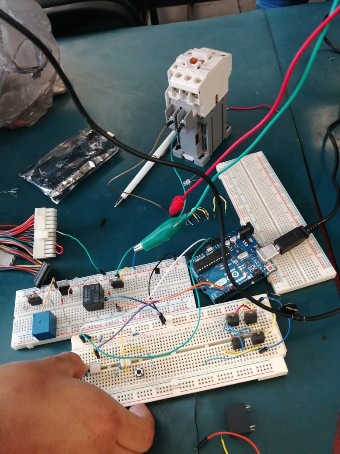
\includegraphics[scale=0.50]{8.png}
\end{figure}

\textbf{ENCLAVE}

\begin{figure}[hbtp]
\centering
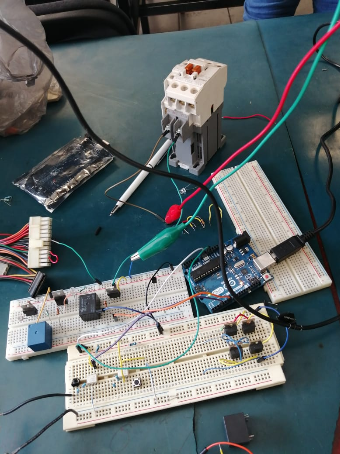
\includegraphics[scale=0.50]{9.png}
\end{figure}

\textbf{DESENCLAVE}

\footnote{Universidad Politécnica De La Zona Metropolitana De Guadalajara} 

\newpage

\section{Conclusión}

El aprendizaje obtenido en esta practica fue como funciona este componente "Darlington" en todos sus aspectos, para esto se observo el datasheet y reviso las características de uso para no quemarlo o quemar componentes como el arduino, también el calculo de su activación fue la misma que el transistor. Este componente no es muy diferente a los que utilizamos en cuanto a función porque es un transistor lo que es un apagador con control en pocas palabras, pero nos da una idea de los múltiples usos que se le da en la industria y que podemos utilizar en futuros provechos aprovechables para la carrera o profesionalmente.

\bibliography{Referencia}
\begin{thebibliography}{X}

\bibitem{Baz} \textsc{THE DECCA DIGITAL.} \textit{Electrónica de  potencia.}Multiplexación.

\bibitem{Baz} \textsc{MANCINI, GINO.} \textit{Modulación por impulsos codificados.} 
Mastering System (2007).

\bibitem{Baz} \textsc{HODGES, DAVID A. (1999).} \textit{Darlintong's - Contributions To Transistor Circuit Desing.} 
IEEE Transactions on Circuits and Systems-I: Fundamental Theory and Applications.

\bibitem{Baz} \textsc{HOROWITZ, PAUL; WINFIELD HILL (1989).} \textit{The Art of electronics.} 
Cambridge University Press. ISBN 0-521-37095-7.


\end{thebibliography}

\bibliographystyle{plain}





\end{document}